\chapter{Solution}
\label{cha:solution}

In this chapter the suggested solution will be detailed, approaching its different components and how they interact between them. The process of generating an \ac{API} based on a \ac{XSD} file contents is complex, so in order to simplify it it was divided into two smaller projects, each one with a given goal and responsibilities. The two main responsibilities in this process are parsing the information from the \ac{XSD} file and generating the \ac{API} based on that same parsed information, which means that the code generation project will have a dependency on the parsing project. For writing purposes the projects will be further referenced by their name, the parsing project being named \hyperref[sec:xsdparser]{XsdParser} and the code generation project named \hyperref[sec:xsdasm]{XsdAsm}.

\section{XsdParser} % (fold)
\label{sec:xsdparser}

XsdParser is a library that parses a \ac{XSD} file into a list of java objects. Each different \ac{XSD} tag has a corresponding Java class and the  attributes of a given \ac{XSD} type are represented as fields in Java. All these classes derive from the same abstract class, XsdAbstractElement. All Java representations of the \ac{XSD} elements follow the schema definition for \ac{XSD} elements\footnote{\url{http://www.datypic.com/sc/xsd/s-xmlschema.xsd.html}}. For example, the xsd:annotation tag only allows xsd:appinfo and xsd:documentation as children nodes, and also can have an attribute named id, therefore XsdParser has the following class:

\lstset{language=Java}
\begin{minipage}{\linewidth}
\begin{lstlisting}[caption={XsdAnnotation class (simplified)},captionpos=b]
public class XsdAnnotation extends XsdIdentifierElements {

    //The id field is inherited from XsdIdentifierElements.
    private List<XsdAppInfo> appInfoList = new ArrayList<>();
    private List<XsdDocumentation> documentations = new ArrayList<>();
}
\end{lstlisting}
\end{minipage}

\subsection{Parsing Strategy}
\label{sec:parsingstrategy}

In order to perform the parsing of the file itself two options were researched, \ac{DOM} and \ac{SAX}. Having balanced the functionalities of both libraries the choice ended up being \ac{DOM}. This choice was based mostly on the fact that \ac{SAX} is an event driven parser and \ac{DOM} is a tree based parser, which is more adequate for the present issue. \ac{DOM} is a library that maps \ac{HTML}, \ac{XHTML} and \ac{XML} files into a tree structure composed by multiple elements, also named nodes. This is exactly what the XsdParser requires in order to obtain all the information from the \ac{XSD} files, which is described in \ac{XML}. 

\noindent
This means that XsdParser uses \ac{DOM} to parse the \ac{XSD} file into a node list, performing a single read on the \ac{XSD} file, in order to avoid multiple reads on the file, which is less efficient. The parsing then follows by iterating on this list and obtaining the name of the element represented by that node, e.g. xsd:element or xsd:complexType. The name of the element will be needed in order to perform a lookup search to find the corresponding parsing function. From that moment on each element obtains all its attribute information directly from its node object. Regarding the other elements that may be contained in a given node they are all similarly parsed. The skeleton function existing in the shared XsdAbstractElement class will iterate in all the children of a given node, invoke the respective parse function of each one and then notify the parent element, using the Visitor pattern, so that the parent element can perform the changes needed based on the element received.

\lstset{
	language=XML,
	morekeywords={xsd:element, xsd:complexType, id}
}

\begin{minipage}{\linewidth}
\begin{lstlisting}[caption={Parsing Concrete Example},captionpos=b]
<xsd:element>
		<xsd:complexType id="complexId">
				(...)	
		</xsd:complexType>
</xsd:element>
\end{lstlisting}
\end{minipage}

\noindent
Based on the abstract explanation given above a more detailed one will be given detailing how the short snippet of \ac{XSD} code will be parsed by the XsdParser. 

Step 1 - DOM parsing:

\noindent
The parsing starts with the \ac{DOM} parsing of the example above, which returns a node list containing only one node, the xsd:element node. Using the xsd:element string the XsdElement parse function will be obtained from an existent string to function mapper. 

Step 2 - XsdElement Attribute Parsing:

\noindent
The XsdElement parse function receives the Node object and extracts all the attribute information, which in this case is empty since the element has no attributes. 

Step 3 - XsdElement Children:

\noindent
In order to parse the XsdElement children the XsdAbstractElement xsdParseSkeleton function is called and starts to iterate in the xsd:element node children, which is a node list containing a single element, the xsd:complexType node. 

Step 4 - XsdComplexType Attribute Parsing:

\noindent
The parsing of the xsd:complexType is similar to the xsd:element, it extracts the attribute information from its respective node, in this case meaning that it will obtain a value from the node attribute named id and assigning it to the id field of the XsdCompleType object. 

Step 5 - XsdElement Visitor Notification:

\noindent
After the parsing of the xsd:compleType node is complete the previously created XsdElement is notified that it contains the newly created XsdCompleType object using the Visitor pattern. The XsdElement should then act accordingly based on the type of the object received as his children, since different types of objects should be treated differently. 

\noindent
This whole behaviour is shared by all the classes that represent a \ac{XSD} element. The Visitor pattern is a very important tool in the parsing process since it allows each element to define a different behaviour for each element received as children. This is also useful to implement the schema rules, since it can also be used to not perform any change if any given element receives other element as children that it shouldn't receive, effectively ignoring the elements that violate the schema specification. The same happens to the attributes present in the parsed \ac{DOM} nodes, each XsdParser object only extracts the attributes defined in the \ac{XSD} schema specification, ignoring other attributes present.

\subsection{Reference solving}
\label{sec:refsolving}

After performing the parsing process described previously, there is still an issue to solve regarding the references that exist in the \ac{XSD} schema definition. In \ac{XSD} files the usage of the ref attribute is frequent in order to avoid repetition of \ac{XML} code. This generates two main problems when handling reference solving, the first one being existing elements with ref attributes referencing non existent elements in the file and the other being the replacement of the reference object by the referenced object when it is present. In order to effectively help resolve the referencing problem there were added some wrapper classes. These wrapper classes contain the wrapped element and serve as a classifier for the wrapped element. The existing wrapper classes are as follow:

\begin{itemize}  
	\item UnsolvedElement - A wrapper class to each element that was not found in the file.
	\item ConcreteElement - A wrapper class to each element that is present in the file.
	\item NamedConcreteElement - A wrapper class to each element that is present in the file and has a name attribute present.
	\item ReferenceBase - A common interface between UnsolvedReference and ConcreteElement.
\end{itemize}

\noindent
Having these wrappers allows for a detailed filtering of the parsed elements which is helpful in the reference solving process. That process starts by obtaining all the NamedConcreteElement objects since they may or may not be referenced by an UnsolvedReference object. The second step is to obtain all the UnsolvedReference objects and iterate them in order to obtain the value of each element ref attribute and perform a lookup search on the NamedConcreteElement objects obtained previously. This is achieved by comparing the value present in the UnsolvedReference ref attribute with the NamedConcreteElement name attribute. If a match is found then XsdParser performs a copy of the object wrapped by the NamedConcreteElement and replaces the element wrapped in the UnsolvedReference object that served as a placeholder. Below it is presented a concrete example of how this process works in order to provide a better understanding of this process.

\lstset{
	language=XML,
	morekeywords={encoding, xsd:schema, xmlns, xmlns:xsd, xsd:group, xsd:choice, id, name,  ref}
}

\begin{minipage}{\linewidth}
\begin{lstlisting}[caption={Reference Solving Example},captionpos=b]
<?xml version='1.0' encoding='utf-8' ?>
<xsd:schema xmlns='http://schemas.microsoft.com/intellisense/html-5' xmlns:xsd='http://www.w3.org/2001/XMLSchema'>
	
		<!-- NamedConcreteType wrapping a XsdGroup -->
		<xsd:group id="replacement" name="flowContent">
				(...)
		</xsd:group>
	
		<!-- ConcreteElement wrapping a XsdChoice -->
		<xsd:choice>
				<!-- UnsolvedReference wrapping a XsdGroup -->
				<xsd:group id="toBeReplaced" ref="flowContent"/>
		</xsd:choice>
</xsd:schema>
\end{lstlisting}
\end{minipage}

\noindent
In this short example we have a XsdChoice element that contains a XsdGroup element with a reference attribute. When replacing the UnsolvedReference objects the XsdGroup with the ref attribute is going to be replaced by a copy of the already parsed XsdGroup with the name attribute. This is achieved by accessing the parent of the element, in this case accessing the parent of the XsdGroup with the ref attribute, in order to remove the element identified by "toBeReplaced" and adding the element identified by "replacement".

\noindent
Having created these classes it is expected that at the end of a successful file parsing only ConcreteElement and/or NamedConcreteElement objects remain. In case there are any remainder UnsolvedReference objects the user can query the parser to discover which elements are missing and where were they used. The user can then correct the missing elements by adding them to the \ac{XSD} file and repeat the parsing process or just acknowledge that those elements are missing. 

\section{XsdAsm} % (fold)
\label{sec:xsdasm}

XsdAsm is a library dedicated to generate a fluent java API based on a XSD file. It uses the previously introduced XsdParser library to parse the \ac{XSD} file contents into a list of Java elements that XsdAsm will use in order to obtain the information needed to generate the correspondent classes. In order to generate classes this library also uses the ASM\footnote{\url{http://asm.ow2.org/}} library, which is a library that provides a Java interface to bytecode manipulation, which allows for the creation of classes, methods, etc. This was the suggested library to implement the code generation part of the project. It is a library that is still regularly maintained, the most recent version, 6.1, was release in 11 march of 2018. Also it has some tools to help the new users to understand how the library works, which are very helpful in order to start generating code and to increase the complexity of the generated code.

\subsection{Supporting Infrastructure}
\label{sec:supportinginfrastructure}

Based on the \ac{XSD} language it was created a infrastructure that served as a common set of classes that will belong to every \ac{API} generated by this project. This supporting infrastructure is divided into three different groups of classes:

Element classes:

\begin{itemize}  
	\item Element - An interface that serves as a base to every parsed \ac{XSD} element.
	\item AbstractElement - An abstract class from all the \ac{XSD} element derive. This class implements most of the methods present on the Element interface.
\end{itemize}

Attribute classes:

\begin{itemize}  
	\item Attribute - An interface that serves as a base to every parsed \ac{XSD} attribute.
	\item BaseAttribute - A class that implements the Attribute interface and adds restriction verification to all the deriving classes. All the attributes that have restrictions should derive from this class.
\end{itemize}

Visitor classes:

\begin{itemize}
	\item ElementVisitor - An interface to define methods for all the generated elements that can be visited with the Visitor pattern.
	\item AbstractElementVisitor - An abstract class that implements all the methods from ElementVisitor, pointing every method implementation for a single method. It helps the end user to create a custom Visitor with less code in situations where only few elements have different implementations.
\end{itemize}

\noindent
Taking in consideration those classes, a very simplistic \ac{API} could be represented with the \ac{UML} diagram (see Figure \ref{img:infrastructure}). In this example we have an element, Html, that extends AbstractElement and an attribute, AttrManifestString that extends BaseAttribute. 

\begin{figure}[ht]
	\centering
	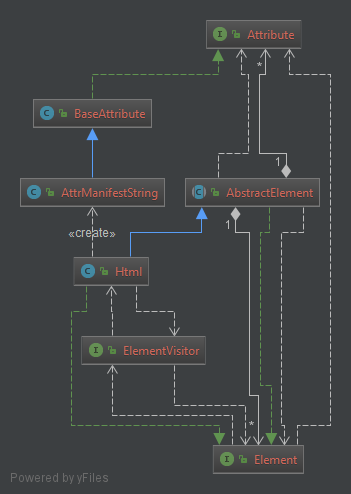
\includegraphics[width=0.8\textwidth]{infrastructure}
	\caption{API - Supporting Infrastructure}
	\label{img:infrastructure}
\end{figure}

\subsection{Code Generation Strategy}
\label{sec:codegenerationstrategy}

In order to understand how most of this project works an example is provided and an detailed explanation will be provided. In this example there will be some simplifications in order to make it easier to understand.

\lstset{
	language=XML,
	morekeywords={xs:element, name, xs:complexType, xs:choice, ref, xs:attributeGroup, xs:attribute, type}
}

\begin{minipage}{\linewidth}
\begin{lstlisting}[caption={Code Generation XSD Example},captionpos=b]
<xs:element name="html">
    <xs:attributeGroup name="commonAttributeGroup">
        <xs:attribute name="someAttribute" type="xs:string">
    </xs:attributeGroup>

    <xs:complexType>
        <xs:choice>
            <xs:element ref="body"/>
            <xs:element ref="head"/>
        </xs:choice>
        <xs:attributeGroup ref="commonAttributeGroup" />
        <xs:attribute name="manifest" type="xs:string" />
    </xs:complexType>
</xs:element>
\end{lstlisting}
\end{minipage}

\noindent
With this example there are a multitude of classes that will need to be created, apart from the always present supporting infrastructure as presented above. 

\begin{itemize}
	\item Html Element - A class that represents the Html element, deriving from AbstractElement.
	\item Body and Head Methods - Both methods present in the Html class that add Body and Head instances to Html children.
	\item Manifest Method - A method present in Html class that adds an instance of the Manifest attribute to the Html attribute list.
\end{itemize}

\lstset{language=Java}

\begin{lstlisting}[caption={Html Element Class},captionpos=b]
public class Html extends AbstractElement implements CommonAttributeGroup {
    public Html() { }
    
    public Html attrManifest(String attrManifest) {
        this.addAttr(new AttrManifest(attrManifest));
    }
    
    public Body body() { this.addChild(new Body()); }
        
    public Head head() { this.addChild(new Head()); }
}
\end{lstlisting}

\begin{itemize}
	\item Body and Head classes - Classes for both Body and Head elements, similar to the generated Html class. The class contents will be dependent on the contents present in the concrete xsd:elements.
\end{itemize}

\bigskip

\begin{minipage}{\linewidth}
\begin{lstlisting}[caption={Body Element Class},captionpos=b]
public class Body extends AbstractElement {
	//Similar to Html, based on the contents of the respective xsd:element node.
}
\end{lstlisting}
\end{minipage}

\bigskip

\begin{minipage}{\linewidth}
\begin{lstlisting}[caption={Head Element Class},captionpos=b]
public class Head extends AbstractElement {
	//Similar to Html, based on the contents of the respective xsd:element node.
}
\end{lstlisting}
\end{minipage}

\begin{itemize}
	\item Manifest Attribute - A class that represents the Manifest attribute, deriving from BaseAttribute.
\end{itemize}

\bigskip

\begin{minipage}{\linewidth}
\begin{lstlisting}[caption={Manifest Attribute Class},captionpos=b]
public class AttrManifestString extends BaseAttribute<String> {
   public AttrManifestString(String attrValue) {
      super(attrValue);
   }
}
\end{lstlisting}
\end{minipage}

\begin{itemize}
	\item CommonAttributeGroup Interface - An interface with default methods that add the group attributes to the concrete element.
\end{itemize}

\bigskip

\begin{minipage}{\linewidth}
\begin{lstlisting}[caption={CommonAttributeGroup Interface},captionpos=b]
public interface CommonAttributeGroup extends Element {

   default Html attrSomeAttribute(String attributeValue) {
      this.addAttr(new SomeAttribute(attributeValue));
      return this;
   }
}
\end{lstlisting}
\end{minipage}

%TODO Maybe add some more stuff here?

\subsection{Restriction Validation}
\label{sec:restrictionvalidation}

In the description of any given \ac{XSD} file there are many restrictions in the way the elements are contained in each other and which attributes are allowed. Reflecting those same restrictions to the Java language we have two ways of ensure those same restrictions, either at runtime or in compile time. This library tries to validate most of the restrictions in compile time, as shown in the example above. But in some restrictions it isn't possible to validate in compile time, an example of this is the following restriction:

\bigskip

\lstset{
	language=XML,
	morekeywords={xs:schema, xs:element, name, xs:complexType, xs:attribute, name, type, xs:simpleType, xs:restriction, xs:maxLenght,
	xs:minLenght, value, xs:list, itemType}
}

\begin{minipage}{\linewidth}
\begin{lstlisting}[caption={Restrictions Example},captionpos=b]
<xs:schema>
    <xs:element name="testElement">
        <xs:complexType>
            <xs:attribute name="intList" type="valuelist"/>
        </xs:complexType>
    </xs:element>
    
    <xs:simpleType name="valuelist">
        <xs:restriction>
            <xs:maxLength value="5"/>
            <xs:minLength value="1"/>
        </xs:restriction>
        <xs:list itemType="xsd:int"/>
    </xs:simpleType>
</xs:schema>
\end{lstlisting}
\end{minipage}

\noindent
In this example we have an element that has an attribute called valueList. This attribute has some restrictions, it is represented by a xs:list and its element count should be between 1 and 5. Transporting this example to the Java language it will result in the following class:

\bigskip

\lstset{language=Java}

\begin{minipage}{\linewidth}
\begin{lstlisting}[caption={Attribute Class Example},captionpos=b]
public class AttrIntList extends BaseAttribute<List> {
   public AttrManifest(List<Integer> list) {
      super(list);
   }
}
\end{lstlisting}
\end{minipage}

\noindent
But with this solution the xs:maxLength and xs:minLength are ignored. To solve this problem the existing restrictions existing in any given attribute are hardcoded in the class static constructor, which stores the restrictions in a Map object. This way, whenever an instance is created a validation function is called in the BaseAttribute constructor and will throw an exception if any restriction present in the Map is violated. This way the generated \ac{API} ensures that any successful usage follows the rules previously defined.

\subsubsection{Enumerations}
\label{sec:enumarations}

In regard to the restrictions there is a special restriction that can be enforced at compile time, the xs:enumeration. In order to obtain that validation at compile time the XsdAsm library generates Enum classes that contain all the values indicated in the xs:enumeration tags. In the following example we have an attribute with three possible values, command, checkbox and radio.

\bigskip

\lstset{
	language=XML,
	morekeywords={xs:attribute, xs:simpleType, xs:restriction, base, xs:enumeration, value}
}

\begin{minipage}{\linewidth}
\begin{lstlisting}[caption={Enumeration Definition},captionpos=b]
<xs:attribute name="type">
    <xs:simpleType>
        <xs:restriction base="xsd:string">
            <xs:enumeration value="command" />
            <xs:enumeration value="checkbox" />
            <xs:enumeration value="radio" />
        </xs:restriction>
    </xs:simpleType>
</xs:attribute>
\end{lstlisting}
\end{minipage}

\noindent
This results in the creation of an Enum, EnumTypeCommand, as shown and the attribute will then receive an instance of EnumTypeCommand, ensuring only allowed values are used.

\bigskip

\lstset{language=Java}

\begin{minipage}{\linewidth}
\begin{lstlisting}[caption={Enumeration Class},captionpos=b]
public enum EnumTypeCommand {
   COMMAND(String.valueOf("command")),
   CHECKBOX(String.valueOf("checkbox")),
   RADIO(String.valueOf("radio"))
}
\end{lstlisting}
\end{minipage}

\begin{minipage}{\linewidth}
\begin{lstlisting}[caption={Attribute Receiving An Enumeration},captionpos=b]
public class AttrTypeEnumTypeCommand extends BaseAttribute<String> {
   public AttrTypeEnumTypeCommand(EnumTypeCommand attrValue) {
      super(attrValue.getValue());
   }
}
\end{lstlisting}
\end{minipage}

\newpage

\subsection{Element Binding}
\label{sec:elementbinding}

In order to support repetitive tasks over an element binders were implemented. This allows for users to define, for example, templates for a given element. An example is presented below, it uses the \ac{HTML}5 \ac{API} as example.

\bigskip

\begin{minipage}{\linewidth}
\begin{lstlisting}[caption={Attribute Receiving An Enumeration},captionpos=b]
public class BinderExample{
    public void bindExample(){
        Html<Html> root = new Html<>();
        Body<Html<Html>> body = root.body();
        
        Table<Body<Html<Html>>> table = body.table();
        table.tr().th().text("Title");
        table.<List<String>>binder((elem, list) ->
                        list.forEach(tdValue ->
                            elem.tr().td().text(tdValue)
                        )
                    );
        
        //Keep adding elements to the body of the document.
    }
}
\end{lstlisting}
\end{minipage}

\noindent
In this example a table is created, and a title is added in the first row as a title header. In regard to the values present in the table instead of having them inserted right away it is possible delay that insertion by indicating what will the element do when the information is received. This way a template can be defined and reused with different values. A full example of how this works is available at the method testBinderUsage. 

\section{Client} % (fold)
\label{sec:client}

Some stuff here.

\section{HtmlFlow}
\label{sec:htmlflow}

More stuff here.
